\documentclass[10pt,twocolumn,letterpaper]{article}

\usepackage{cvpr}
\usepackage{times}
\usepackage{epsfig}
\usepackage{graphicx}
\usepackage{amsmath}
\usepackage{amssymb}
\usepackage{enumitem}
\usepackage[font=footnotesize,skip=3pt]{caption}
\usepackage{subcaption}
\usepackage{adjustbox}
\usepackage{svg}
\usepackage{float}
% Include other packages here, before hyperref.
\DeclareMathOperator*{\argmax}{arg\,max}
\DeclareMathOperator*{\argmin}{arg\,min}
% If you comment hyperref and then uncomment it, you should delete
% egpaper.aux before re-running latex.  (Or just hit 'q' on the first latex
% run, let it finish, and you should be clear).
\usepackage[breaklinks=true,bookmarks=false]{hyperref}

\cvprfinalcopy % *** Uncomment this line for the final submission

\def\cvprPaperID{****} % *** Enter the CVPR Paper ID here
\def\httilde{\mbox{\tt\raisebox{-.5ex}{\symbol{126}}}}

% Pages are numbered in submission mode, and unnumbered in camera-ready
%\ifcvprfinal\pagestyle{empty}\fi
\setcounter{page}{1}

\begin{document}
\setlength{\textfloatsep}{0.7\baselineskip plus 0.2\baselineskip minus 0.5\baselineskip}
\setlength{\abovedisplayskip}{4pt}
\setlength{\belowdisplayskip}{4pt}
\setlength{\abovedisplayshortskip}{0pt}
\setlength{\belowdisplayshortskip}{0pt}
%%%%%%%%% TITLE
\title{Improving State-of-the-Art GAN Video Synthesis}

\author{Michael Gentner\\
TU Munich\\
85748 Garching\\
{\tt\small michael.gentner@tum.de}
% For a paper whose authors are all at the same institution,
% omit the following lines up until the closing ``}''.
% Additional authors and addresses can be added with ``\and'',
% just like the second author.
% To save space, use either the email address or home page, not both
\and
Lars Carius\\
TU Munich\\
85748 Garching\\
{\tt\small lars.carius@tum.de}
}

\maketitle
%\thispagestyle{empty}

%%%%%%%%% ABSTRACT
\begin{abstract}
We propose multiple methods for improving state-of-the-art GAN-based video synthesis approaches. We show that GANs using 3D-convolutions for video generation can easily be extended to predicting coherent depth maps alongside RGB frames, but results indicate that this does not improve RGB accuracy if depth is available. We further propose critic-correction, a method for improving videos generated by latent space curve fitting. Additionally, we study the effect of Principal Component Analysis as well as different backprojection methods on the quality of generated videos. Our code can be found at \url{https://github.com/CariusLars/ImprovingVideoGeneration} .
\end{abstract}

%%%%%%%%% BODY TEXT
\section{Introduction}

Synthesizing high-resolution videos is a highly relevant topic for commercial applications of Generative Adversarial Networks (GANs). The technique can be used for creating animations in games and, at some point, photo-realistic video clips. With the possibility to condition the generated videos on input data, GANs have the potential to outperform classic approaches of video editing and special effects.

%-------------------------------------------------------------------------
\section{Related Work}
Generative Adversarial Networks have been shown to generate high-resolution images that are indistinguishable from real photographs to the human eye \cite{Karras2018a, Karras2018}. The domain of synthesizing coherent high-resolution videos of considerable length remains an open challenge.\\% generation is a substantially harder task that is tackled in current research.\\
BigGAN \cite{Brock2018}, a large architecture for image synthesis, was extended to video generation by Clark {\em et\ al.} using Recurrent Neural Network (RNN) blocks and separate discriminators for spatial and temporal consistency \cite{Clark2019}. 
Building on Progressively Growing GANs (PGGANs) \cite{Karras2018}, Aigner and K\"orner used 3D-convolutions to synthesize video sequences conditioned on input frames \cite{Aigner2019}. Other approaches include 
\begin{figure}[H]
	\centering
	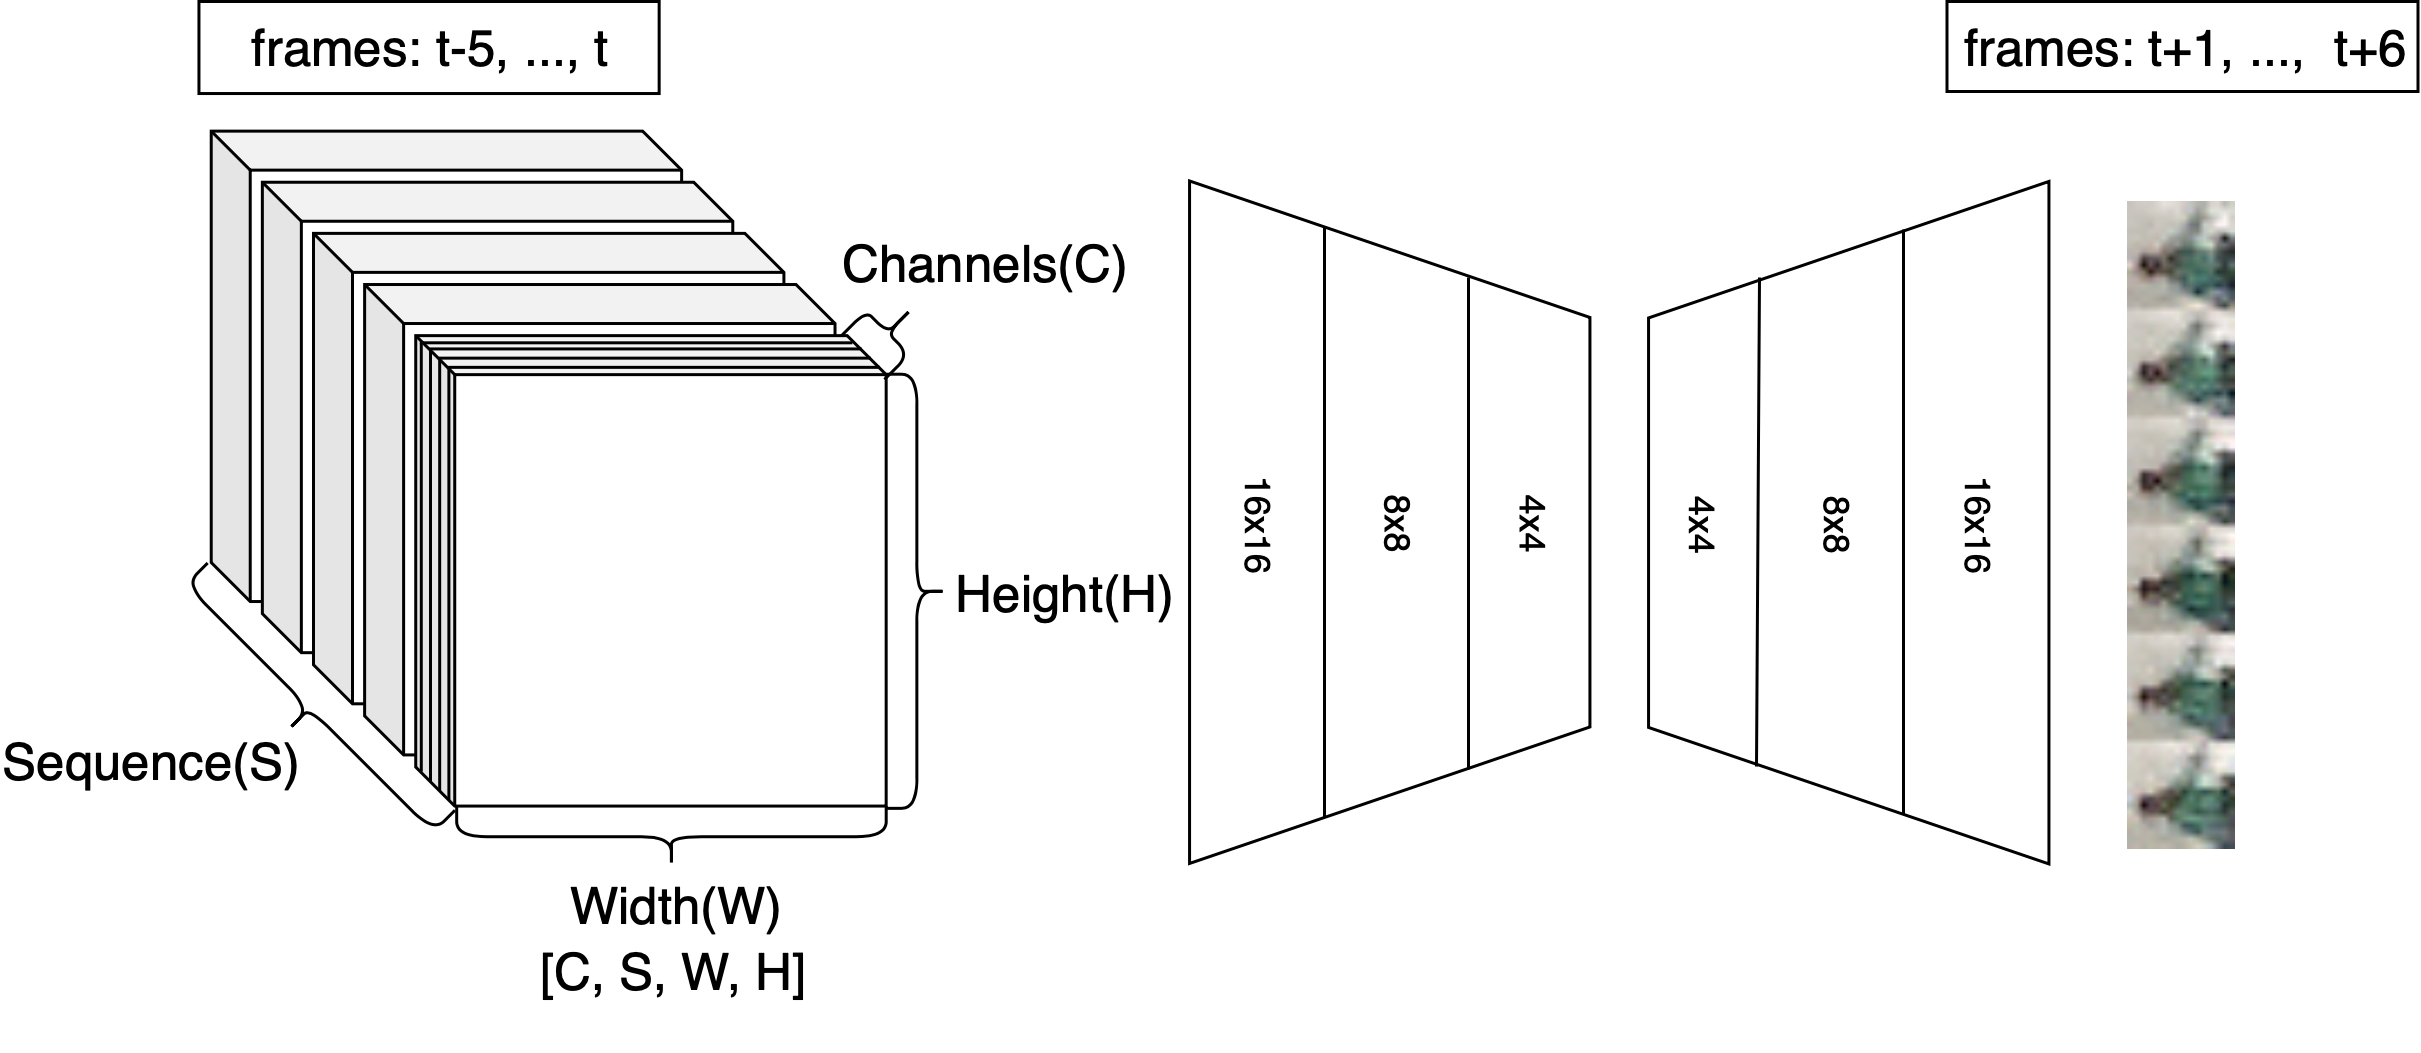
\includegraphics[width=0.5\textwidth]{graphics/FutureGAN/FutureGAN.png}
	\caption{3D-convolutional video generation pipeline adapted from \cite{Aigner2019}. 6 RGB/RGB-D frames serve as conditioning input, the network generates the consecutive 6 RGB/RGB-D frames. Every 20 epochs, encoder and decoder are grown to learn features on all resolutions (see \cite{Karras2018})}
	\label{fig:futuregan}
\end{figure}
explicit modeling of back- and foreground dynamics to achieve spatio-temporal consistency \cite{Vondrick2016}. None of the approaches consider using depth information. \\
In other research, the low-dimensional latent manifold of GANs has been widely used to interpolate between generated images \cite{Karras2018}. Zhu {\em et\ al.} use encoded spatial properties to morph images based on user suggestions \cite{Zhu2016}, Chen {\em et\ al.} \cite{Chen2019} propose additional methods to manipulate specific properties of generated faces.
\begin{figure*}[]
	\centering
	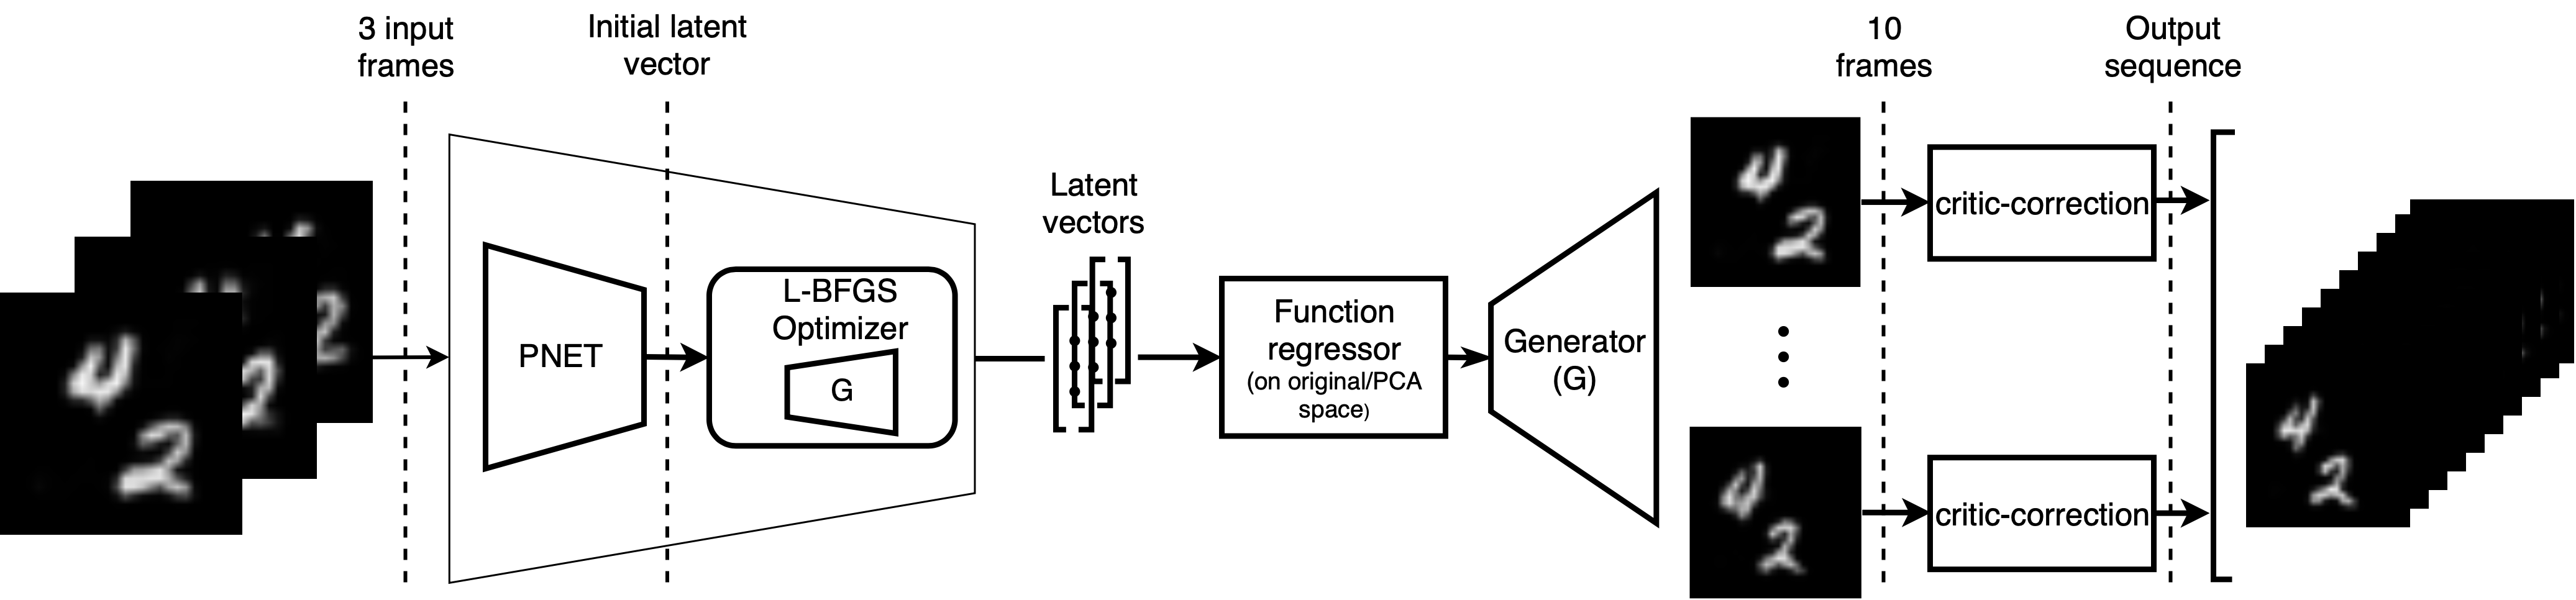
\includegraphics[width=\textwidth]{graphics/LSVG/LSVG.png}
	\caption{Latent space video generation pipeline. Conditioning frames are projected into latent space using a numerical optimizer initialized with a projection network. A polynomial is then fitted to the latent vectors (if the latent space is very large, PCA before regression and backprojection afterwards proved to be useful) and new points are sampled from the curve to generate the output video in latent space. The generator translates the video into image space, critic-correction improves the video in post-processing}
	\label{fig:lsvg}
\end{figure*}
%------------------------------------------------------------------------
\section{Method}
We propose multiple approaches to improve the state-of-the-art of video synthesis:
\begin{itemize}[noitemsep]
	\renewcommand{\labelitemi}{\tiny$\blacksquare$}
	\item Use of depth information to improve the quality of generated videos
	\item Leveraging curve-fitting on the latent space
	\item Improving synthesized videos with critic-correction and Principal Component Analysis (PCA)
\end{itemize} 
\subsection{Incorporating depth}
Due to its promising results, the FutureGAN architecture \cite{Aigner2019} served as a basis for this approach. We incorporated depth by adding a feature channel containing depth maps normalized to $[-1,1]$ (see figure \ref{fig:futuregan}). From the dense RGB-D dataset generated by Nie\ss ner {\em et\ al.}, we extracted video snippets of 12 frames each from which the first 6 served as conditioning input frames and the remaining 6 as ground truth for the generated video. We used 40\% of frames per sequence as test set. We limited the progressive growing of the network to a maximum resolution of 16$\times$16 px, trained for 20 epochs in each resolution step and adapted the batch size after each resolution change to best utilize the available GPU memory. \\
We tested the hypothesis of depth information improving the synthesized video quality by allowing to learn spatio-temporal correlations in an ablation study.

\subsection{Latent Space Video Generation}

We performed video synthesis on MovingMNIST by fitting curves to the latent manifold of a GAN. We propose critic-correction as a postprocessing method for the generated video. Conditioning on input frames is incorporated by backprojecting given images into latent space utilizing optimization techniques and a projection network, the entire pipeline is visualized in figure \ref{fig:lsvg}.

\subsubsection{GAN-Architecture} 
We adapted the DCGAN architecture of \cite{DCGAN} to incorporate the WGAN-GP loss of \cite{Gulrajani2017}. This remedies the diligent training of standard GANs. We used instance normalization \cite{INST} to render the network agnostic to high contrast images found in MovingMNIST. 

\subsubsection{Backprojection}
The projection of input frames into latent space is necessary to achieve conditioning of the generated videos. Inspired by Zhu {\em et\ al.}, we used a combination of L-BFGS optimization and a projection network \cite{Zhu2016}. We fed an input image $\mathbf{x}$ into our projection network $P$ (P-net) which was trained to minimize the binary cross-entropy loss between $\mathbf{x}$ and the image generated from the predicted latent vector $\mathbf{z}$. The weights of the generator network $G(P(\mathbf{x}))$ were frozen and $P$ closely resembles the structure of the critic used in the initial GAN training. The latent vector generated by $P$ is used as an initialization for the numerical solver. 

\subsubsection{Critic-Correction}
Due to imperfect manifolds and backprojections, generated frames were often close to the desired image, yet still blurry. We propose the new technique critic-correction to compensate for this. The critic determines the realism of images generated from $z$, so we used it to optimize our obtained latent vectors. Fixing the parameters of critic $C$ and generator $G$ and using stochastic gradient descent to optimize the latent vector $z$, the update rule is given by:

\begin{align}
\mathbf{z}_{i+1} = \mathbf{z}_{i} - \alpha \nabla_{\mathbf{z}} \left[-  \mathbb{E}[C(G(\mathbf{z}_i))] \right]
\end{align}

\subsubsection{Regression in Latent Space}
The projections of input images into the latent space serve as conditioning input. Parametrized by time, polynomials are fitted to the individual dimensions of the samples in latent space. The curves are evaluated at new points in time to synthesize a latent video sample. We assumed that certain properties correspond to certain dimensions in the manifold. Therefore, we applied PCA on the input projections, fitted a curve in the principal component space and applied the inverse projection to the output to reconstruct the original space. We compared these results to approaches without PCA.
%------------------------------------------------------------------------
\section{Results}
We conducted separate experiments for both approaches. We summarize our findings below, additional samples can be found in our repository. 
\subsection{Extending FutureGAN}
\begin{table}[H]
	\centering
	\begin{adjustbox}{max width=0.5\textwidth}
		\begin{tabular}{lllll}
			& RGB$\rightarrow$RGB & RGB-D$\rightarrow$RGB & RGB$\rightarrow$RGB-D & RGB-D$\rightarrow$RGB-D \\ \hline
			MSE        & \textbf{0.0656}       & 0.0686                  & 0.0765                  & 0.0749                    \\
			PSNR       & \textbf{18.2980}      & 18.1068                 & 12.7094                 & 17.7737                   \\
			SSIM       & \textbf{0.6452}       & 0.6321                  & 0.6290                  & 0.6188                    \\
			Depth MSE  & -                     & -                       & 0.0669                  & \textbf{0.0582}           \\
			Depth PSNR & -                     & -                       & 20.2700                 & \textbf{20.9937}          \\ \hline
		\end{tabular}
	\end{adjustbox}
	\caption{Scores of the different methods to incorporate depth information into the FutureGAN architecture. The networks predict 6 consecutive frames based on 6 conditioning frames}
	\label{tab:ablation_scores}
\end{table}
\begin{figure}[]
	\begin{subfigure}[b]{0.5\textwidth}
		\centering
		
\includegraphics[width=\textwidth]{graphics/ground_truth.png}
	\end{subfigure}
	\begin{subfigure}[b]{0.5\textwidth}
		\centering
		
\includegraphics[width=\textwidth]{graphics/nodepth.png}
	\end{subfigure}
	\begin{subfigure}[b]{0.5\textwidth}
		\centering
		
\includegraphics[width=\textwidth]{graphics/depth_in.png}
	\end{subfigure}
	\begin{subfigure}[b]{0.5\textwidth}
		\centering
		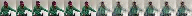
\includegraphics[width=\textwidth]{graphics/depth_out.png}
	\end{subfigure}
	\begin{subfigure}[b]{0.5\textwidth}
		\centering
		
\includegraphics[width=\textwidth]{graphics/depth.png}
	\end{subfigure}
	\caption{Test set sequence from the ablation study. Each row represents a video sequence with 6 input frames (conditioning) and 6 frames predicted by the network. From top to bottom: ground truth, RGB$\rightarrow$RGB, RGB-D$\rightarrow$RGB, RGB$\rightarrow$RGB-D, RGB-D$\rightarrow$RGB-D}
	\label{fig:ablation_images}
\end{figure}

Figure \ref{fig:ablation_images} shows an example sequence analysed in the ablation study, table \ref{tab:ablation_scores} summarizes the performance of tested architectures. While the baseline performed best on the RGB channels, low test set errors were achieved on the predicted depth maps in the corresponding approaches.
On the one hand, this supports the fact that depth information is not used by the network to infer information about the RGB predictions. On the other hand, the findings show that depth predictions can be learned just as easily as RGB channels. The small increase in RGB error in approaches generating depth shows that additionally learning depth predictions comes at very little cost and can, within given constraints of a suitable training set, even be accomplished without depth input being available at test time.
\subsection{Latent Space Video Generation}
\begin{figure}[]
	\begin{subfigure}[b]{0.11\textwidth}
		\centering
		
\includegraphics[width=\textwidth]{graphics/backprojection/bfgs/0.png}
		\caption{L-BFGS}
	\end{subfigure}
	\begin{subfigure}[b]{0.11\textwidth}
		\centering
		
\includegraphics[width=\textwidth]{graphics/backprojection/pnet/0.png}
		\caption{P-net}
	\end{subfigure}
	\begin{subfigure}[b]{0.11\textwidth}
		\centering
		
\includegraphics[width=\textwidth]{graphics/backprojection/pnet_bfgs/0.png}
		\caption{Both}
	\end{subfigure}
	\begin{subfigure}[b]{0.11\textwidth}
		\centering
		
\includegraphics[width=\textwidth]{graphics/backprojection/original/0.png}
		\caption{Ground Truth}
	\end{subfigure}
	\caption{Comparison of backprojection methods: a) L-BFGS-optimization b) Projection learned by convolutional neural network c) L-BFGS with initialization by network b d) ground truth. The projections produce latent vectors, for visualization they are fed into the generator to obtain images}
	\label{fig:backprojection}
\end{figure}

While the backprojection of test set images into the latent space using L-BFGS-optimization worked well for large latent space dimensions (128 or 256), it performed poorly with reasonable latent space sizes (16). Training a convolutional network for the backprojection task yielded better results, combining both approaches by initializing the L-BFGS-solver with the network outperformed both individual methods significantly (see figure \ref{fig:backprojection}). Additional experiments using different numerical solvers did not improve performance.
\begin{figure}[]
	\centering
	\begin{subfigure}[b]{0.11\textwidth}
		\centering
		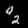
\includegraphics[width=\textwidth]{graphics/d_correction/ground_truth/8.png}
		\caption{Before corr.}
	\end{subfigure}
	\begin{subfigure}[b]{0.11\textwidth}
		\centering
		\includegraphics[width=\textwidth]{graphics/d_correction/d_cor/8.png}
		\caption{After corr.}
	\end{subfigure}
	\begin{subfigure}[b]{0.11\textwidth}
		\centering
		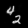
\includegraphics[width=\textwidth]{graphics/d_correction/ground_truth/7.png}
		\caption{Before corr.}
	\end{subfigure}
	\begin{subfigure}[b]{0.11\textwidth}
		\centering
		
\includegraphics[width=\textwidth]{graphics/d_correction/d_cor/7.png}
		\caption{After corr.}
	\end{subfigure}
	\caption{Critic correction applied to frames generated by the video synthesis pipeline. Image a) is successfully corrected to image b), the algorithm fails on image c) and results in a digit error displayed in d). The ground truth contains the numbers 4 and 2}
	\label{fig:critic_correction}
\end{figure}

Our proposed method of critic-correction produced mixed results. As figure \ref{fig:critic_correction} shows, the correction leads to significantly sharper output images and often converges to the correct numbers. In some cases, difficult to interpret numbers converged to wrong digits. In future works, this could be compensated with additional information transfer from surrounding frames (in the time dimension).
\begin{figure}[]
	\centering
	\begin{subfigure}[b]{0.038\textwidth}
		\centering
		
\includegraphics[width=\textwidth]{graphics/interpolation_linear/0.png}
	\end{subfigure}	
	\begin{subfigure}[b]{0.038\textwidth}
		\centering
		
\includegraphics[width=\textwidth]{graphics/interpolation_linear/1.png}
	\end{subfigure}
	\begin{subfigure}[b]{0.038\textwidth}
		\centering
		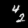
\includegraphics[width=\textwidth]{graphics/interpolation_linear/2.png}
	\end{subfigure}
	\begin{subfigure}[b]{0.038\textwidth}
		\centering
		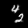
\includegraphics[width=\textwidth]{graphics/interpolation_linear/3.png}
	\end{subfigure}
	\begin{subfigure}[b]{0.038\textwidth}
		\centering
		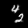
\includegraphics[width=\textwidth]{graphics/interpolation_linear/3.png}
	\end{subfigure}
	\begin{subfigure}[b]{0.038\textwidth}
		\centering
		
\includegraphics[width=\textwidth]{graphics/interpolation_linear/4.png}
	\end{subfigure}
	\begin{subfigure}[b]{0.038\textwidth}
		\centering
		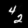
\includegraphics[width=\textwidth]{graphics/interpolation_linear/5.png}
	\end{subfigure}
	\begin{subfigure}[b]{0.038\textwidth}
		\centering
		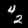
\includegraphics[width=\textwidth]{graphics/interpolation_linear/6.png}
	\end{subfigure}
	\begin{subfigure}[b]{0.038\textwidth}
		\centering
		
\includegraphics[width=\textwidth]{graphics/interpolation_linear/7.png}
	\end{subfigure}
	\begin{subfigure}[b]{0.038\textwidth}
		\centering
		\includegraphics[width=\textwidth]{graphics/interpolation_linear/8.png}
	\end{subfigure}
	\begin{subfigure}[b]{0.038\textwidth}
		\centering
		
\includegraphics[width=\textwidth]{graphics/interpolation_linear/9.png}
	\end{subfigure}
	

	\caption{Synthesized video sequence based on 3 conditioning input frames. Regression to a linear curve and critic correction were used for the generation process}
	\label{fig:output_sequence}
\end{figure}

On the simple MovingMNIST dataset, videos generated by interpolating the backprojected conditioning frames in latent space led to reasonably coherent output sequences (Figure \ref{fig:output_sequence}). Regression to a polynomial of rank 1 produced the best results with the fewest digit errors, critic correction reduced blurriness significantly but led to occasional mistakes in the digits. PCA before regression hardly changed the results for a 16-dimensional latent space but did significantly improve the video quality for a 256-dimensional latent space. This indicates that it helps to alleviate the problem of poorly-conditioned latent spaces in video generation tasks.

%------------------------------------------------------------------------
\section{Conclusion}
	Our experiments indicate that with the given FutureGAN architecture, depth information does not improve RGB video prediction performance. Predicting depth maps, however, comes at reasonable accuracy with very low cost, which is valuable especially for robotics tasks. \\
	Our contributions to video generation by leveraging smooth latent spaces include multiple methods to compensate for instabilities and noise in the regression of latent vectors and confirm the results of previous papers. In a set of constraint applications, both critic-correction and applying PCA before regression improved the synthesized videos.
%------------------------------------------------------------------------
{\small
\bibliographystyle{ieee_fullname}
\bibliography{vidgan}
}

\end{document}